\section{Regression}

The concepts discussed in the following section could also be presented in
random variables instead of sample ones. As the geometry of sample variables
is almost of no difference comparing to the random ones, the logic of
all the theorems is also the same.


\subsection{Geometry of sample variables}

\marginnote{
\begin{multline*}
\sCorr(x,y) = \frac{\sCov(x,y)}{\sqrt{\sVar(x)\sVar(y)}} \\
= \frac{\frac{1}{n-1}\sum_{i=1}^n (x_i - \bar x)(y_i - \bar y)}{\sqrt{\frac{1}{n-1} \sum_{i=1}^n (y_i - \bar y)\frac{1}{n-1} \sum_{i=1}^n (\hat y_i - \bar{\hat y})}}
\end{multline*}
}

In the~same manner which was performed in Section~\ref{rvs}, we define
the~scalar product of two sample variables
$x =
\begin{pmatrix}
x_1 \\
\vdots \\
x_n
\end{pmatrix}$
and
$y =
\begin{pmatrix}
y_1 \\
\vdots \\
y_n
\end{pmatrix}$
as a sample covariation between them:
\[
\langle x, y \rangle = \sCov(x, y).
\]
The main characteristics of a~vector are its length and direction.
Again, we introduce the~length
\[
\sqrt{\sCov(x,x)} = \sqrt{\sVar(x)} = \sigma_x
\]
and the~angle between two sample variables
\[
\cos(x,y) = \frac{\sCov(x,y)}{\sqrt{\sVar(x)\sVar(y)}} = \sCorr(x,y).
\]
Note that from the definition of the angle
it follows that the~sample correlation coefficient can range from $-1$ to $1$.

\begin{marginfigure}
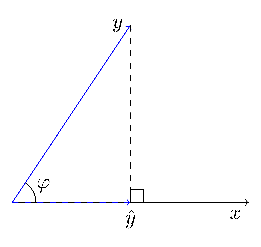
\includegraphics[scale=0.85]{figures/02_basic_projection.pdf}
\caption{Vector $y$ projected onto vector $x$.}
\label{fig:corr_proj}
\end{marginfigure}

Completely analogus to the~case of random variables,
the projection of such a sample variable $y$ onto
$\{cx| c \in \mathbb{R}\}$ is $\hat y = \sCorr(x,y) \cdot y$.

Looking at Figure~\ref{fig:corr_proj}, we can interpret the~square of sample correlation coefficient.
Using the fact that $cos^2 \varphi$ is the~squared ratio of
the~leg adjacent to $\varphi$ to hypotenuse, we can conclude that
\[
\sCorr^2(x,y) = \frac{\sVar(\hat y)}{\sVar(y)},
\]
as the variance of a vector is associated with the square of its length.
Thus, the~sample correlation coefficient squared shows
the~fraction of variance in $y$ which can be explained
with the~most similar vector proportional to $x$.


\subsection{Sample correlation when a constatnt vector added}

\marginnote{
\begin{align*}
\sCorr(x + \alpha \mathbf{1}, y) &= \frac{\sCov(x + \alpha \mathbf{1}, y)}{\sVar(x + \alpha \mathbf{1}) \sVar(y)} \\
&= \frac{\sCov(x,y)\sCov(\alpha \mathbf{1},y)}{\sVar(x)\sVar(y)} \\
&= \frac{\sCov(x,y)}{\sVar(x)\sVar(y)} \\
&= \sCorr(x,y)
\end{align*}
}

\begin{theorem}
Adding a~vector of constants does not affect the sample correlation coefficient:
\[
\sCorr(x + \alpha \mathbf{1}, y) = \sCorr(x,y)
\]
where $\alpha \in \mathbb{R}$.
\end{theorem}

\begin{proof}
Firstly, we project vectors $x$ and $y$ onto $Lin^{\perp}(\mathbf{1})$
in order to get $x^c = x - \bar x$ and $y^c = y - \bar y$ (`c' stands for `centred').
It can be shown that the~matrix corresponding to projecting onto the line spanned by
a~vector of all ones has the~following form
\[
\frac{\mathbf{1}^T \mathbf{1}}{\mathbf{1} \mathbf{1}^T} = \frac{\begin{pmatrix} 1 & \ldots & 1 \end{pmatrix} \begin{pmatrix} 1 \\ \vdots \\ 1 \end{pmatrix}}{\sum_{i=1}^n 1} = \begin{pmatrix} \frac{1}{n} & \ldots & \frac{1}{n} \\ \vdots & \ddots & \vdots \\ \frac{1}{n} & \ldots & \frac{1}{n} \end{pmatrix}
\]
Thus, projecting onto the~orthogonal subspace is equivalent to
substracting the~projected vector, i.e., the vector of averages, from the original one.

\begin{marginfigure}
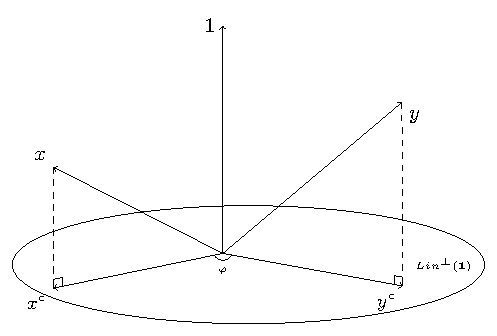
\includegraphics[scale=0.65]{figures/02_correlation_constant_centered_variables.pdf}
\caption{Centred vectors $x^c$ and $y^c$}
\label{fig:corr_xyc}
\end{marginfigure}

Also note that the~angle $\varphi$ between the~original and centred vectors remains the~same.
The~result of this step is shown in Figure~\ref{fig:corr_xyc}.

Then we need to derive a new vector $\tilde x$ with constants added to each component.
Geometrically adding a vector of costants means adding a vector of all ones
scaled by $\alpha \in \mathbb{R}$, i.e., $\alpha \mathbf{1}$.
Then the new vector $\tilde x$ can be broken up into a sum of $\alpha \mathbf{1}$ and
$\beta x$, $\alpha, \beta \in \mathbb{R}$, which can be seen in Figure~\ref{fig:corr_tildex}.
After that we will project this new vector $\tilde x$ onto $Lin^{\perp}(\mathbf{1})$.
By the properties of projection it is of no difference whether to project
the whole vector $\tilde x$ or project its parts $\alpha \mathbf{1}$
and $\beta x$ — the result is the same.
So, while $\beta x$ is projected onto the span of $x^c$, the projection of $\alpha \mathbf{1}$
onto the orthohgonal space $Lin^{\perp}(\mathbf{1})$ yields zero as demonstrated
in Figure~\ref{fig:corr_tildex}.
Moreover, it follows that the angle between $\tilde x$ and $y$ is still $\varphi$.

\begin{figure}
  \centering
  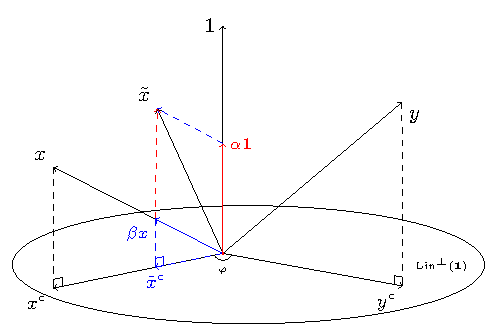
\includegraphics[width=0.6\linewidth]{figures/02_correlation_constant_decomposition.pdf}
  \caption{Decomposition and projection of $\tilde x$}
  \label{fig:corr_tildex}
\end{figure}

Finally, putting everything together we finish the proof:
\[
\sCorr(x + \alpha \mathbf{1}, y) = \sCorr(x,y)
\]

\begin{figure}
  \centering
  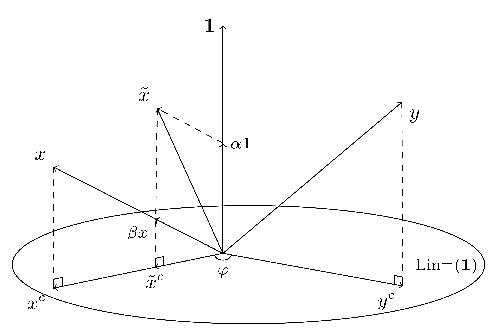
\includegraphics[width=0.6\linewidth]{figures/02_correlation_constant_proof.pdf}
  \caption{$\sCorr(x + \alpha \mathbf{1}, y) = \sCorr(x,y)$ as the corresponding angles are equal.}
  \label{fig:corr_final}
\end{figure}
\end{proof}


\subsection{Sample correlation coefficient in simple linear regression}

\marginnote{
Assuming the underlying relationship between $x$ and $y$ to be
\[
y_i = \beta_1 + \beta_2 x_i + \varepsilon_i \quad i=1,\ldots,n
\]
where $\varepsilon_i$ is an error term the following holds
\begin{align*}
\sCorr(y, \hat y) &= \frac{\sCov(y)\sCov(\hat y)}{\sqrt{\sVar(y)\sVar(\hat y)}} \\
&= \frac{\sCov(y)\sCov(\hat \beta_1 + \hat \beta_2 x)}{\sqrt{\sVar(y)\sVar(\hat \beta_1 + \hat \beta_2 x)}} \\
&= \frac{\sCov(y)\sCov(\hat \beta_2 x)}{\sqrt{\sVar(y)\sVar(\hat \beta_2 x)}} \\
&= \frac{\hat \beta_2 \sCov(y)\sCov(x)}{|\hat \beta_2| \sqrt{\sVar(y)\sVar(x)}} \\
&= sign(\hat \beta_2) \frac{\sCov(y)\sCov(x)}{\sqrt{\sVar(y)\sVar(x)}}
\end{align*}
}

\begin{theorem}
A linear regression model with one explanatory variable and constant term
\[
y = \beta_1 + \beta_2 x + \varepsilon
\]
has the property
\[
\sCorr(y, \hat y) = sign(\hat \beta_2) \sCorr(y, x)
\]
\end{theorem}

\begin{proof}
Firstly, we consider the case when $\hat \beta_2 > 0$ and introduce the base
picuture of the proof as depicted in Figure~\ref{fig:corr_pos_base}.
It has been shown earlier that the correlation coefficient represents the angle
betweem two random vectors.
So in order to complete the proof we need to find the appropriate angles and compare them.

%\begin{figure}[h!]
%\center{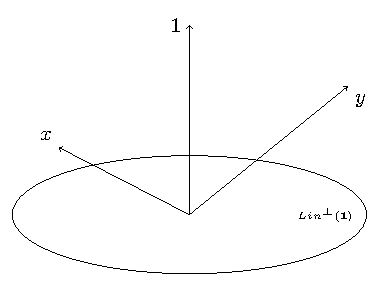
\includegraphics[width=0.35\linewidth]{figures/02_simple_regression_coefficient_basic.pdf}}
%\caption{Vectors $x$, $y$ and $\mathbf{1}$.}
%%\label{fig:corr_pos_base}
%\setfloatalignment{b}
%\end{figure}

However, it seems to be difficult to compare the angles in the three dimensional space.
That is why we start with projecting both $x$ and $y$ onto the space perpendicular to the vector of all ones $\mathbf{1}$ as shown in Figure~\ref{fig:corr_pos_xyc}.
We denote this space as $Lin^{\perp}(\mathbf{1})$. The resulting vectors are $x - \bar x \cdot \mathbf{1}$  and $y - \bar y \cdot \mathbf{1}$ respectively
since projection of any vector $\vec{a}$ on the line given by a vector of all ones yields the vector of averages $\vec{\bar a}$.

\begin{marginfigure}[3\baselineskip]
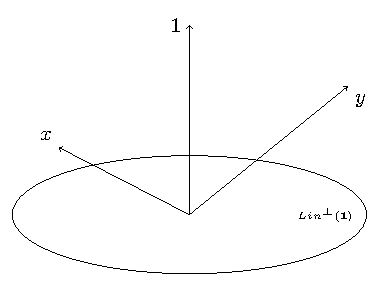
\includegraphics[scale=0.7]{figures/02_simple_regression_coefficient_basic.pdf}
\caption{Vectors $x$, $y$ and $\mathbf{1}$.}
\label{fig:corr_pos_base}
\end{marginfigure}

In order to get the angle between $y$ and $\hat y$ we should start with regressing $y$ on $Lin(x, \mathbf{1})$.
Then the only thing thing left is to project $\hat y$ onto $Lin^{\perp}\mathbf{1}$ since the $y$ vector has already been projected.
Note that the projected $\hat y$ falls onto tha span of vector $x - \bar x \cdot \mathbf{1}$ as it can be decomposed into a sum $a x + b \mathbf{1}$ where $a, b \in \mathbb{R}$.
$a x$ is projected in the same way as $x$ and $b \mathbf{1}$ yields zero when projected onto the orthogonal space.
The result of this step is shown in Figure~\ref{fig:corr_pos_yhatc}.

\begin{figure*}[h!]
\begin{center}
\subfigure[]{
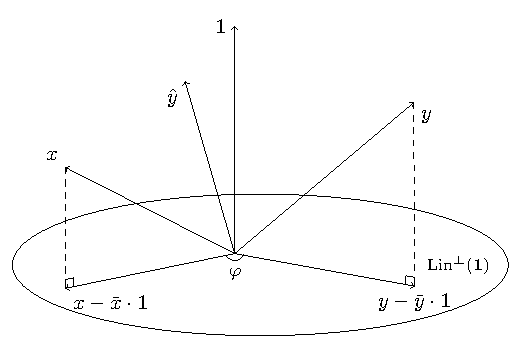
\includegraphics[width=0.45\linewidth]{figures/02_simple_regression_coefficient_centred_variables.pdf}
\label{fig:corr_pos_xyc}}
%\hspace{4ex}
\subfigure[]{
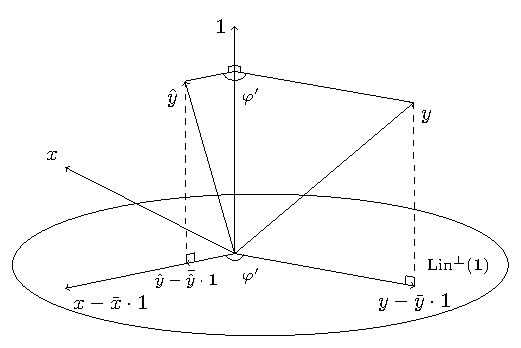
\includegraphics[width=0.45\linewidth]{figures/02_simple_regression_coefficient_yhat_projected.pdf}
\label{fig:corr_pos_yhatc}}
\caption{\subref{fig:corr_pos_xyc}: `Centred' $x$ and $y$, i.e., projected onto $Lin^{\perp}(\mathbf{1})$; \subref{fig:corr_pos_yhatc}: `Centred' $\hat y$, i.e., projected onto $Lin^{\perp}(\mathbf{1})$.}
\end{center}
\end{figure*}

Since the projection of $\hat y$ lies exactly on the span of vector $x - \bar x \cdot \mathbf{1}$, we can conclude that $cos \varphi = \cos \varphi '$ and to put it another way $\sCorr(x,y) = \sCorr(y, \hat y)$.

Now consider the case when $\hat \beta_2 < 0$.
Note that the sign of $\beta_1$ does not influence the correlation coefficient sign.
The only difference is that now $\hat y$ is projected onto the span of  $x - \bar x \cdot \mathbf{1}$ and not on this vector itself while the projections of $x$ and $y$ remain the same.
Looking at Figure~\ref{fig:corr_negative} we deduce that the angle betwween $y$ and $\hat y$ is compelement to the angle between $x$ and $y$.
Using trigonometric properties, we simplify $\cos(180^{\circ} - \varphi) = -\cos\varphi$ which in turn implies $\sCorr(x,y) = -\sCorr(y,\hat y)$.

\begin{figure}[h!]
\begin{center}
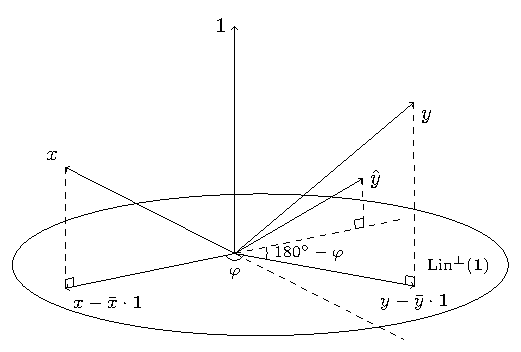
\includegraphics{figures/02_simple_regression_coefficient_negative.pdf}
\label{fig:corr_negative}
\caption{Case of $\beta_2 < 0$.}
\setfloatalignment{b}
\end{center}
\end{figure}
\end{proof}


\subsection{RSS + ESS = TSS}

\marginnote{
Consider a regresion model with $n$ observations and $k$ explanatory variables including a constant unit vector
\[
y = X \beta + \varepsilon
\]
The OLS estimator for the vector of coefficients $\beta$ is
\[
\hat \beta = (X^T X)^{-1} X^T y
\]
and the residual vector is
\begin{align*}
\hat e &= y - \hat y \\
&= y - X \hat \beta \\
&= y - X (X^T X)^{-1} X^T y
\end{align*}
Then we define residual sum of squares (RSS), explained sum of squares (ESS) and total sum of squares (TSS) as follows:
\begin{align*}
RSS &= \lVert y - \hat y \rVert^2_2 \\
ESS &= \lVert \hat y - \bar y \rVert^2_2 \\
TSS &= \lVert y - \bar y \rVert \\
\end{align*}
Disclosing parentheses and using the fact that $\hat{y}^T y = \hat{y}^T \hat{y}$
\begin{align*}
\hat{y}^T y &= \beta^T X^T y \\
&=  y^T X (X^T X)^{-1} X^T y \\
\hat{y}^T \hat{y} &= \beta^T X^T X \beta \\
&= y^T X (X^T X)^{-1} X^T X (X^T X)^{-1} X^T y \\
&= y^T X (X^T X)^{-1} X^T y
\end{align*}
we obtain
\begin{align*}
RSS &= y^T y -\hat{y}^T \hat{y} \\
ESS &= \hat{y}^T \hat{y} - \hat{y}^T \bar{y} + \bar{y}^T \bar{y} \\
TSS &= y^T y - 2 y^T \bar y +  \bar{y}^T \bar{y}
\end{align*}
When putting everything together all the terms cancel out which proves
\[
ESS + RSS = TSS
\]
}

\begin{theorem}
A linear regression model with $n$ observations and $k$ explanatory variables including a constant unit vector
\[
y = X \beta + \varepsilon
\]
has the following property
\[
RSS + ESS = TSS
\]
where $RSS = \lVert y - \hat y \rVert^2_2$, $ESS = \lVert \hat y - \bar y \rVert^2_2$, $TSS = \lVert y - \bar y \rVert^2_2$.
\end{theorem}

\begin{proof}
The proof will be presented for the case of two regressor $x$ and $\mathbf{1}$ in order for the picture to be clear.
However, the same logic applies for the case of $k$ regressors.

We start with depicting the vectors $y \in \mathbb{R}^{n-2}$ and $x, \mathbf{1} \in \mathbb{R}^2$.
Then we project $y$ onto $Lin(x, \mathbf{1})$ and obtain $\hat y$ which is shown in Figure~\ref{fig:tss_base}.

From this picture we can immediately derive $\sqrt{RSS}$ as by definition this is the squared difference between $y$ and $\hat y$.

\begin{figure}[h!]
\begin{center}
\subfigure[]{
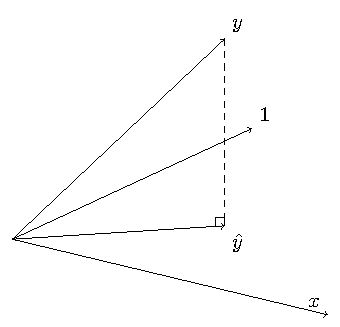
\includegraphics[width=0.4\linewidth]{figures/02_rss_ess_tss_yhat.pdf}
\label{fig:tss_base} }
\hspace{4ex}
\subfigure[]{
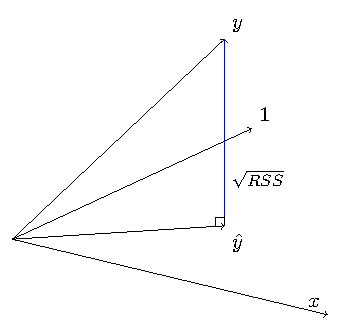
\includegraphics[width=0.4\linewidth]{figures/02_rss_ess_tss_sqr_rss.pdf}
\label{fig:tss_rss}}
\caption{\subref{fig:tss_base}: Vectors $y \in \mathbb{R}^{n-2}$ and $\hat y \in Lin(x, \mathbf{1})$; \subref{fig:tss_rss}: Residual sum of squares.}
\end{center}
\end{figure}

So as to visualize $ESS$ and $TSS$ we first need to visualize vector of averages $\bar y$.
Geometrically this means projecting a vector onto a line spanned by vector $\mathbf{1}$.

Now we both project $y$ and $\hat y$ onto $\mathbf{1}$ and following the definition obtain $\sqrt{TSS}$ as the difference vector $y - \bar y$ and $\sqrt{ESS}$ as the vector $\hat y - \bar y$.

\begin{figure}[h!]
\begin{center}
\subfigure[]{
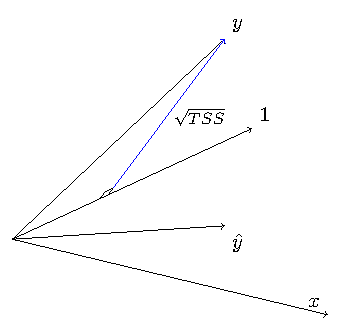
\includegraphics[width=0.4\linewidth]{figures/02_rss_ess_tss_sqr_tss.pdf}
\label{fig:tss_tss}}
\hspace{4ex}
\subfigure[]{
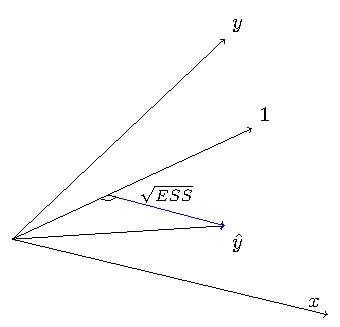
\includegraphics[width=0.4\linewidth]{figures/02_rss_ess_tss_sqr_ess.pdf}
\label{fig:tss_ess}}
\caption{\subref{fig:tss_tss}: Total sum of squares; \subref{fig:tss_ess}: Explained sum of squares.}
\end{center}
\end{figure}

\begin{marginfigure}
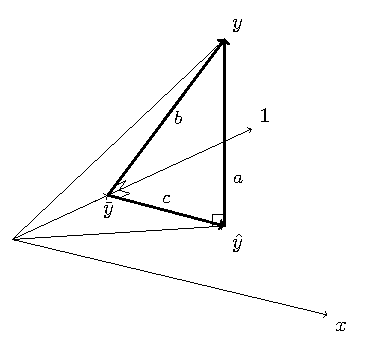
\includegraphics[scale=0.7]{figures/02_rss_ess_tss_final.pdf}
\caption{$(\sqrt{RSS})^2 + (\sqrt{ESS})^2 = (\sqrt{TSS})^2$}
\label{fig:tss_final}
\end{marginfigure}

The final step is to put everything together.
Note that since $y - \hat y$ is perpendicular to $Lin(x, \mathbf{1})$ it is also perpendicular to $\hat y - \bar y$ and $\mathbf{1}$ as these vectoros are in $Lin(x, \mathbf{1})$.
Then, applying the theorem of three perpendiculars we conclude that the foot of vector $y - \bar y$ is the same point as the foot of the vector $\hat y - \bar y$.
Thus, we obtain a right angle triangle and can apply the Pythagorean theorem for the catheti $\sqrt{RSS}$ and $\sqrt{ESS}$ and the
hypotenuse $\sqrt{TSS}$:
\[
(\sqrt{RSS})^2 + (\sqrt{ESS})^2 = (\sqrt{TSS})^2
\]
\end{proof}


\subsection{Determination coefficient}

\marginnote{
\begin{multline*}
\sCorr^2(y,\hat y) = \left(\frac{\sCov(y, \hat y)}{\sqrt{\sVar(y)\sVar(\hat y)}}\right)^2 \\
= \frac{\sCov(y, \hat y) \sCov(y, \hat y)}{\sVar(y)\sVar(\hat y)} \\
= \frac{\sCov(\hat y + e, \hat y) \sCov(\hat y + e, \hat y)}{\sVar(y)\sVar(\hat y)} \\
= \frac{(\sCov(\hat y, \hat y) + \sCov(e, \hat y))(\sCov(\hat y, \hat y) + \sCov(e, \hat y))}{\sVar(y)\sVar(\hat y)} \\
= \frac{\sVar(\hat y) \sVar(\hat y)}{\sVar(y)\sVar(\hat y)} = \frac{\sVar(\hat y)}{\sVar(y)} = \frac{ESS}{TSS} = R^2
\end{multline*}
}

\begin{theorem}
A linear regression model with $n$ observations and $k$ explanatory variables including a constant unit vector
\[
y = X \beta + \varepsilon
\]
has the following property
\[
R^2 = \sCorr^2(y, \hat y)
\]
\end{theorem}

\begin{proof}
Proving this theorem geometrically means showing that the determination coefficient can be interpreted as some squared angle
which happens to be eqaul to the squared angle betwen $y$ and $\hat y$.

Consider Figure~\ref{fig:tss_final} from the previous proof.
It was shown there that the vectors $y - \bar y$, $y - \hat y$ and $\hat y - \bar y$ form a right triangle.
Having defined the determination coefficient as
\[
R^2 = \frac{ESS}{TSS}
\]
we conclude that its geometric interpretaion is
\[
R^2 = \frac{ESS}{TSS} = \cos^2 \varphi
\]
as shown in Figure~\ref{fig:r_sq_angle}.

\begin{figure}
  \center{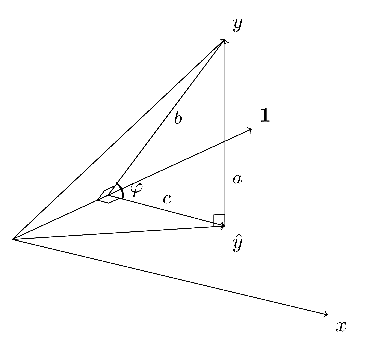
\includegraphics{figures/02_determination_coefficient.pdf}}
  \caption{Determination coefficient as squared $\cos \varphi$}
  \label{fig:r_sq_angle}
\end{figure}

Recall that the sample correlation coefficient two vectors was defined earlier as the angle between these two vectors.
Thus, we conclude that $\sCorr(y, \hat y)$ is the angle between $y$ and $\hat y$ which is also eqaul to $\cos \varphi$.
Finally, squaring both sides, we obtain
\[
R^2 = \sCorr^2(y, \hat y)
\]
\end{proof}


\subsection{Regression line and point of averages}

\marginnote{
If the regression contains the intercept, the following equation holds:
\begin{align*}
\hat y  &= X \hat \beta \\
&= X (X^T X)^{-1} X^T y \\
&= X (X^T X)^{-1} X^T X \beta + X (X^T X)^{-1} X^T \varepsilon
\end{align*}
Premultiplying both sides by $X^T$, we obtain:
\begin{align*}
X^T \hat y &=  X^T X (X^T X)^{-1} X^T X \beta \\
&+ X^T X (X^T X)^{-1} X^T \varepsilon \\
&= X^T X \beta + X^T \varepsilon
\end{align*}
This is a system of equations. The first row of $X^T$ is $\mathbf{1}$ vector, so we can write out the first equation:
\[
\sum_{i=1}^n \hat y_i = \sum_{i=1}^{n} \sum_{j=1}^{k} x_{ij} \beta_{j}
\]
From the first equation in the system
\[
X^T \hat y = X^T y
\]
we obtain
\[
\sum_{i=1}^{n} \hat y_i = \sum_{i=1}^{n} y
\]
And this finishes the proof:
\[
\frac{1}{n} \sum_{i=1}^{n} y = \frac{1}{n} \sum_{i=1}^{n} \sum_{j=1}^{k} x_{ij} \beta_{j}
\]
}

\begin{theorem}
In a linear regression model with one explanatory variable and constant term
\[
y = \beta_1 + \beta_2 x + \varepsilon
\]
the point of averages lies on the estimated regression line.
\end{theorem}

\begin{proof}
For the geometrical proof it suffices to show that $\hat y$ is a linear combination of the regressors, which is true by construction,
and that $\frac{1}{n} \sum_{i=1}^{n} \hat y_i = \frac{1}{n} \sum_{i=1}^{n} y$. In order for the pictures to be more clear the proof will be presented for the case of two regressors.

The first step is regressing $y$ on $Lin(\mathbf{1}, x)$. As shown in Figure~\ref{fig:averages_lin}, we obtain $\hat y$ as a linear combination of $\mathbf{1}$ and $x$.
The next step is to regress both $y$ and $\hat y$ on $\mathbf{1}$ which results in $\bar y$ and $\bar \hat y$ correspondingly.
By the theorem of three perpendiculars, $\bar y = \bar \hat y$ which is shown in Figure~\ref{fig:averages_bars}.

\begin{figure}[ht!]
\begin{center}
\subfigure[]{
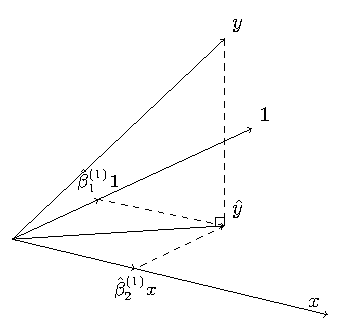
\includegraphics[width=0.4\linewidth]{figures/02_averages_yhat_decomposed.pdf}
\label{fig:averages_lin} }
\hspace{4ex}
\subfigure[]{
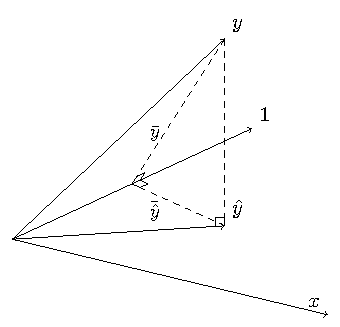
\includegraphics[width=0.4\linewidth]{figures/02_averages_final.pdf}
\label{fig:averages_bars}}
\caption{\subref{fig:averages_lin}: Regression of $y$ on $Lin(\mathbf{1},x)$; \subref{fig:averages_bars}: Regression of $y$ and $\hat y$ on $\mathbf{1}$.}
\end{center}
\end{figure}
\end{proof}


\subsection{Frisch–Waugh–Lovell theorem}

\marginnote{From regresison~\ref{eq:fwl_2} we get the following estimator:
\begin{align*}
\hat\beta_2 &= ((M_1 X_2)^T M_1 X_2)^{-1}(M_1 X_2)^T M_1 y \\
&= (X_2^T M_1^T M_1 X_2)^{-1}  X_2^T M_1^T M_1 y \\
&= (X_2^T M_1 X_2)^{-1}  X_2^T M_1 y
\end{align*}
As for regresison~\ref{eq:fwl_1}, let us note that due to $y = \hat y + \hat u$ $y$ can be decomposed as follows:
\[
y = Py + My = X_1 \hat \beta_1 + X_2 \hat \beta_2 + My
\]
Premultiplying both sides by $X_2^T M_1$, we obtain:
\begin{align*}
X_2^T M_1 y &= X_2^T M_1 X_1 \hat\beta_1 + X_2^T M_1 X_2 \hat\beta_2 + X_2^T M_1 M y \\
&=  X_2^T M_1 X_2 \hat\beta_2 + X_2^T M_1 M y \\
&= X_2^T M_1 X_2 \hat\beta_2
\end{align*}
On the last step we used the fact that
\begin{align*}
(X_2^T M_1 M y)^T = y^T M^T M_1^T X_2 \\
= y^T M M_1 X_2 = y^T M X_2 = 0^T
\end{align*}
Assuming $X_2^T M_1 X_2$ is invertible, we get the same estimator
\[
\hat\beta_2 = (X_2^T M_1 X_2)^{-1}  X_2^T M_1 y
\]
}

\begin{theorem}
Consider regression
\begin{equation} \label{eq:fwl_1}
y = X_1 \beta_1 + X_2 \beta_2 + u
\end{equation}
where $X_{n \times k} = [X_1 X_2]$, i.e. $X_1$ consists of first $k_1$ columns of $X$ and $X_2$ consists of remaining $k_2$ columns of $X$,
$\beta_1$ and $\beta_2$ are comfortable, i.e. $k_1 \times 1$ and $k_2 \times 1$ vectors.
Consider another regresison
\begin{equation}  \label{eq:fwl_2}
M_1 y = M_1 X_2 \beta_2 + M_1 u
\end{equation}
where $M_1 = I - P_1$ projects onto the~orthogonal complement of the~column space~of
$X_1$ and $P_1 = X_1(X_1^TX_1)^{-1}X_1^T$ is the~projection onto the~column space of~$X_1$.
Then the~estimate of $\beta_2$ from regression~\ref{eq:fwl_1} will be the~same
as the~estimate from regression~\ref{eq:fwl_2}.
\end{theorem}

There are two ways to~visualize the~proof of~the~Frisch-Waugh-Lovell theorem
using geometric concepts. Both are presented below.

\begin{proof}
1.~Consider the following model:
\begin{equation} \label{eq:fwl_proof}
y_i = \beta_1 x_i + \beta_2 z_i + u_i
\end{equation}

We start with regression `all-at-once' and will distinct its coefficients with~index $(1)$.
The~only step in~obtaining $\beta_1^{(1)}$ is regressing $y$ on~$Lin(x,z)$ and
then expanding $\hat y$ as a~linear combination of~basis vectors $x$ and $z$,
which is shown in~Figure~\ref{fig:fwl_1_regression_3d}. Figure~\ref{fig:fwl_1_regression_lin}
depicts $Lin(x, z)$.

\begin{figure}[ht!]
\begin{center}
\subfigure[]{
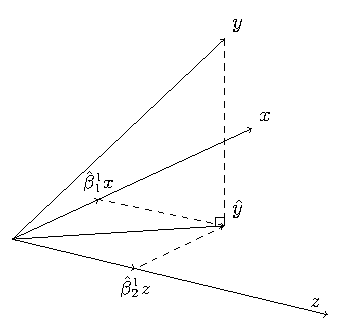
\includegraphics[width=0.4\linewidth]{figures/02_fwl_v1_yhat_decomposed.pdf}
\label{fig:fwl_1_regression_3d} }
\hspace{4ex}
\subfigure[]{
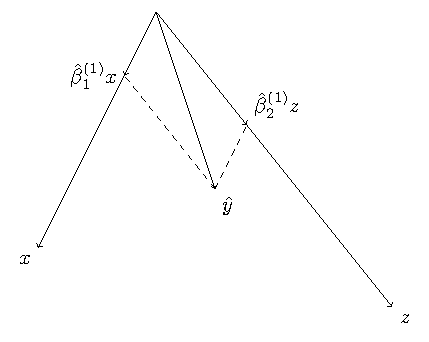
\includegraphics[width=0.4\linewidth]{figures/02_fwl_v1_yhat_decomposed_lin.pdf}
\label{fig:fwl_1_regression_lin}}
\caption{\subref{fig:fwl_1_regression_3d}: Regression of $y$ on $Lin(x,z)$; \subref{fig:fwl_1_regression_lin}: $Lin(x, z)$.}
\end{center}
\end{figure}

As for the~model~\ref{eq:fwl_2}, where several regressions are performed consecutively,
we start with regressing $y$~on~$z$, resulting in $\tilde{y}$,
which we will refer~to as~`cleansed' $y$.

\begin{equation}\label{eq:fwl_2_y_clean}
\begin{aligned}
y &= \alpha z + \varepsilon \\
\hat\alpha &= \frac{y^T z}{z^T z} \\
\tilde{y} &= \hat\varepsilon = y - \frac{y^T z}{z^T z}z
\end{aligned}
\end{equation}

Following that, $x$ is regressed on $z$, resulting in $\tilde{x}$ — `cleansed' $x$.

\begin{equation}\label{eq:fwl_2_x_clean}
\begin{aligned}
x &= \gamma z + \nu \\
\hat\gamma &= \frac{x^T z}{z^T z} \\
\tilde{x} &= \hat\nu = x - \frac{x^T z}{z^T z}z
\end{aligned}
\end{equation}

Geometric results of these two steps are presented in~\ref{fig:fwl_2_regression_first}.

Finally, `cleansed' $y$ must be regressed on `cleansed' $x$.
However, it cannot be performed immediately as $\tilde{y}$ and $\tilde{x}$ are skew lines.
So at first, we fix this problem by translation and after taht obtain
$\hat\beta_1^{(2)}\tilde x$ (see Figure~\ref{fig:fwl_2_regression_trans}).

\begin{figure}[ht!]
\begin{center}
\subfigure[]{
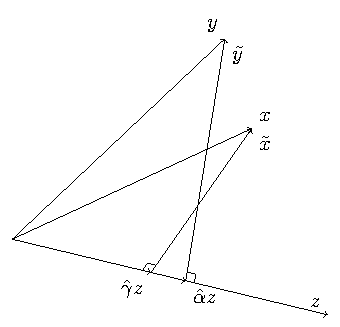
\includegraphics[width=0.4\linewidth]{figures/02_fwl_v1_cleansed_variables.pdf}
\label{fig:fwl_2_regression_first} }
\hspace{4ex}
\subfigure[]{
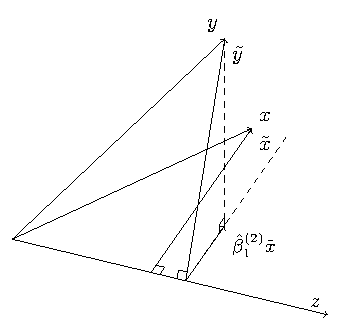
\includegraphics[width=0.4\linewidth]{figures/02_fwl_v1_translation.pdf}
\label{fig:fwl_2_regression_trans}}
\caption{\subref{fig:fwl_2_regression_first}: Regression of $y$ on $z$ and of $x$ on $z$;
\subref{fig:fwl_2_regression_trans}: Translation of $\tilde{x}$.}
\end{center}
\end{figure}

Now, let us picture all the results in one figure and mark some main points.

\begin{figure}[ht!]
\begin{center}
\subfigure[]{
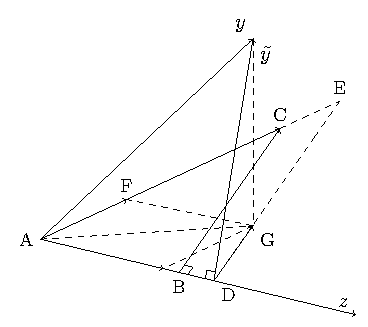
\includegraphics[width=0.4\linewidth]{figures/02_fwl_v1_final.pdf}
\label{fig:fwl_3_3d} }
\hspace{4ex}
\subfigure[]{
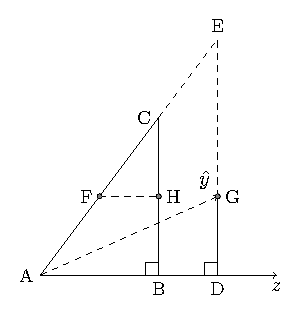
\includegraphics[width=0.4\linewidth]{figures/02_fwl_v1_final_lin.pdf}
\label{fig:fwl_3_lin}}
\caption{\subref{fig:fwl_3_3d}: Point A stands for the origin, B — $\hat\gamma z$,
C — $x$, D — $\hat\alpha z$, E — intersection of vector $x$ and line parallel to $\tilde x$,
F — $\hat\beta_1^{(1)} x$, G — $\hat\beta_1^{(2)} \tilde{x}$; \subref{fig:fwl_3_lin}: $Lin(x,z)$.}
\end{center}
\end{figure}

In Figure~\ref{fig:fwl_3_lin} segments $AF$ and $BH = DG$ stand for $\hat\beta_1^{(1)}x$
and $\hat\beta_1^{(2)}\tilde x$ respectively, while segments AC and BC represent $x$ and $\tilde{x}$.
Having two congruent angles, triangles ABC and FHC are simillar.
Then, it follows:
\[
\frac{AF}{AC} = \frac{BH}{BC} \Leftrightarrow \frac{\hat\beta_1^{(1)}x}{x} = \frac{\hat\beta_1^{(2)}\tilde x}{\tilde x} \Leftrightarrow \hat\beta_1^{(1)} = \hat\beta_1^{(2)}
\]

2. Alternatively, we could implement a~concept close to the~partial correlation.
In the~same model~\ref{eq:fwl_proof} we wiil treat $z$ vector fixed and again
consecutively cleanse the $x$ and $y$ variables by projecting them onto
the~space orthogonal to $z$, i.e., $Lin^\perp(z)$ as demonstrated in Figure~\ref{fig:fwl_v2_rcleansed}.
Then we perform a~regression of the~`cleansed' $\tilde y$ on the~`cleansed' $\tilde x$
(see Figure\ref{fig:fwl_v2_regression_cleansed}).

\begin{figure}[ht!]
\begin{center}
\subfigure[]{
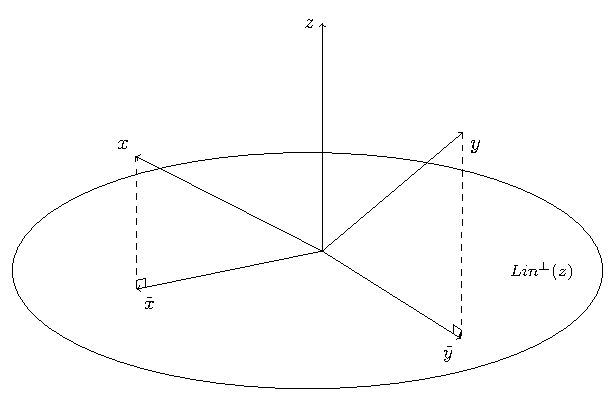
\includegraphics[width=0.45\linewidth]{figures/02_fwl_v2_cleansed_variables.pdf}
\label{fig:fwl_v2_rcleansed}}
\subfigure[]{
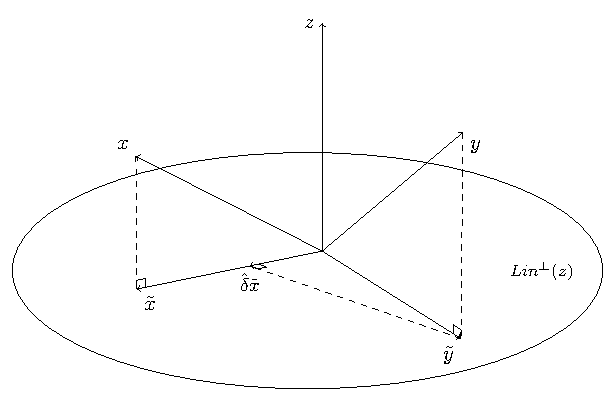
\includegraphics[width=0.45\linewidth]{figures/02_fwl_v2_cleansed_regression.pdf}
\label{fig:fwl_v2_regression_cleansed}}
\caption{\subref{fig:fwl_2_regression_first}: `Cleansed' variables $\tilde x$ and $\tilde y$;
\subref{fig:fwl_2_regression_trans}: `Cleansed' $\tilde y$ regressed on `cleansed' $\tilde{x}$.}
\end{center}
\end{figure}

Now we show that the~latter regression produces $\hat \beta_1$ coefficient which
is exatly the~coefficient from the~`one-step' regression of~original $y$ onto
original $x$ and $z$. Recall that the~vector $y$ can be split~up into a~sum of
some multiple of $x$ and some multiple of $z$. Since the second term is
the~orthogonal component its projection yields zero. The~multiple of $x$
is equal to $\hat \beta_1$ by construction.

Assume that the~coefficient at~$\tilde x$ is some unknown variable $\hat \delta$.
Then consider the~similar triangles in the $Lin(x,z)$. From the~proportions
we obtain:
\[
\frac{CE}{CA} = \frac{CD}{CB} \Leftrightarrow \frac{\hat \beta_1 x}{x} = \frac{\hat \delta \tilde x}{\tilde x} \Rightarrow \hat \beta_1 = \hat \delta
\]

\begin{figure}[ht!]
\begin{center}
\subfigure[]{
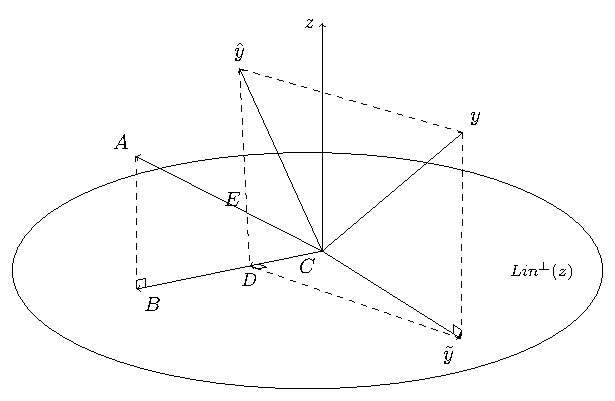
\includegraphics[width=0.45\linewidth]{figures/02_fwl_v2_similar_triangles.pdf}
\label{fig:fwl_v2_triangles}}
\subfigure[]{
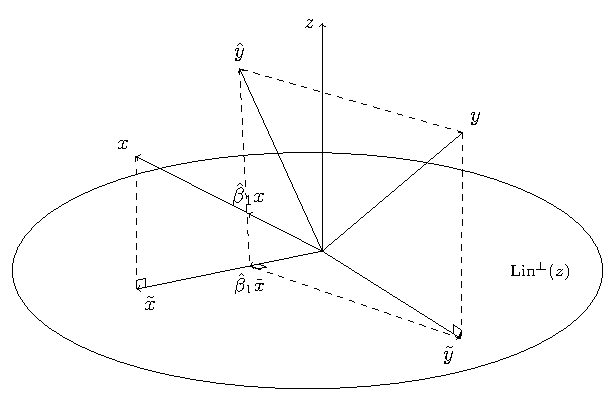
\includegraphics[width=0.45\linewidth]{figures/02_fwl_v2_final.pdf}
\label{fig:fwl_v2_final}}
\caption{\subref{fig:fwl_2_regression_first}: Similar triangles: $\bigtriangleup ABC \sim \bigtriangleup EDC$;
\subref{fig:fwl_2_regression_trans}: Alternative proof for the Frisch-Waugh-Lovell theorem.}
\end{center}
\end{figure}
\end{proof}


\subsection{Duality of regressors and residuals}

The idea of duality is widely used in mathematics.
The concept is two apply some transformation twice and get the~original object.
For example, if $f(a) = 1/a$:
\[
x \stackrel{f}{\to} \frac{1}{x} \stackrel{f}{\to} \frac{1}{1/x} = x
\]
We show that there is duality between regressors and residuals.

\begin{theorem}
Let $x_i$ be a $n \times 1$ regressor,
$u_i$ — a residual in regression of $x_i$ on all the rest regressors,  $i = 1, \ldots, k$.
Consider a transformation of a vector $v$, $f(v) = v/\lVert v \rVert^2$.
Then applying this transformation on the residuals $u_1, \ldots, u_k$ yields
new regressors $v_1, \ldots, v_k$.
Performing $k$ regressions of each $v_i$ on all the rest regressors and
applying the same transformation to the new residuals results in
the original regressors $x_1, \ldots, x_k$.
\end{theorem}

\begin{proof}

We start with $2$-dimensional case with two regressors,
and discuss the~case of spaces of higher dimensions later.

\begin{marginfigure}
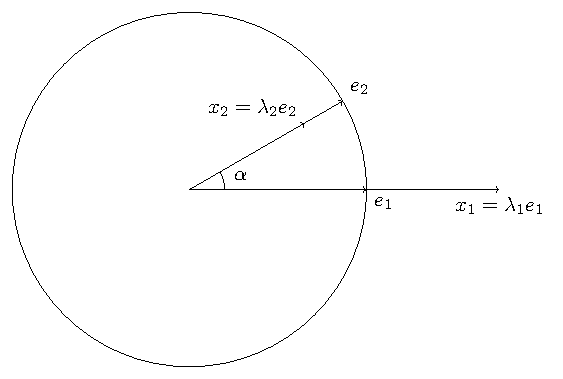
\includegraphics[scale=0.7]{figures/02_duality_original_regressors.pdf}
\caption{Two regressors in the unit circle.}
\end{marginfigure}

As stated in the~theorem we need to keep the~measure of the~lengths of the~regressors.
In order to do this we choose a~basis in $\mathbb{R}^2$ in such a~way that
\begin{align*}
&x_1 = \lambda_1 e_1, \quad \lVert e_1 \rVert = 1 \\
&x_2 = \lambda_2 e_2, \quad \lVert e_2 \rVert = 1
\end{align*}
where $\lambda_1, \lambda_2 \in \mathbb{R}$.

\begin{marginfigure}[2\baselineskip]
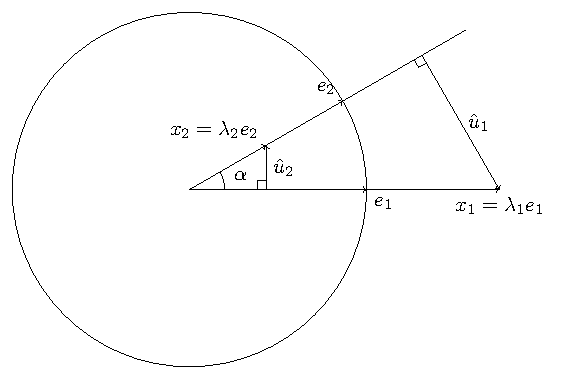
\includegraphics[scale=0.7]{figures/02_duality_first_residuals.pdf}
\label{fig:duality_fst_residuals}
\caption{Residuals $\hat{u}_1$ and $\hat{u}_2$}
\end{marginfigure}

Then we perform two regressions
\begin{align*}
&x_1 = \beta_1 x_2 + u_1 \\
&x_2 = \beta_2 x_1 + u_2
\end{align*}
and get the residuals $\hat{u}_1$, $\hat{u}_2$.
Being orthogonal to $x_2$ and $x_1$ correspondingly, they can be written as follows
\begin{align*}
&\hat{u}_1 = \sin \alpha \cdot \lambda_1 \tilde{e}_1, \quad \lVert \tilde{e}_1 \rVert = 1 \\
&\hat{u}_2 = \sin \alpha \cdot \lambda_2 \tilde{e}_2, \quad \lVert \tilde{e}_2 \rVert = 1
\end{align*}
where $\tilde{e}_1 \perp e_2$ and $\tilde{e}_2 \perp e_1$.

For convinence we translate all the vectors $x_1$, $x_2$, $\hat{u}_1$, $\hat{u}_2$
to the origin of the unit circle as shown in Figure~\ref{fig:duality_fst_residuals_translated}
and after that we invert them.

\begin{marginfigure}
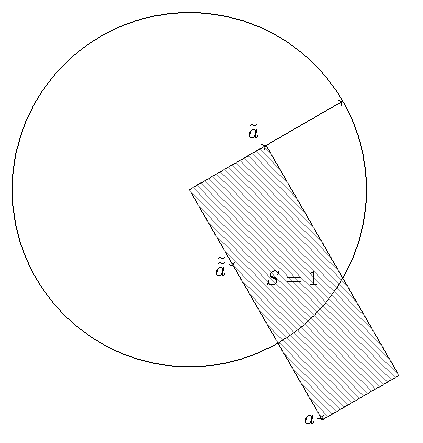
\includegraphics[scale=0.7]{figures/02_duality_inversion.pdf}
\label{fig:duality_inversion}
\caption{Example of inversion for vector $a$.}
\end{marginfigure}

In order to illustrate inversion consider an example with an arbitrary vector $a$.
Knowing its length, the aim is to find such an orthogonal vector $\tilde a$
that the product $\lVert a \rVert^2 \cdot \lVert \tilde a \rVert^2 = 1$.
In other words, we need to find an edge of rectangle with area equal to $1$.
Solving for $\tilde a$, we obtain the length of the inverted vector $a$.
The only thing left is to rotate this inverted vector back
to get a vector $\tilde{\tilde a}$ which satisfies both
\begin{align*}
& \lVert \tilde{\tilde a} \rVert^2 = \frac{1}{\lVert a \rVert^2} \\
& \cos(a, \tilde{\tilde a}) = 1
\end{align*}

\marginnote[3\baselineskip]{
The transformation stated in the theorem is $f(v) = v / \lVert v \rVert^2$.
Generally speaking, $g(v) = v / (c \cdot \lVert v \rVert^2)$ where $c \in \mathbb{R}$
would also work.
\begin{multline*}
v \stackrel{g}{\to} \frac{v}{c \cdot \lVert v \rVert^2} = w \stackrel{g}{\to} \\
\frac{w}{c \cdot \lVert w \rVert^2} = \frac{\frac{v}{c \cdot \lVert v \rVert^2}}{c \frac{\lVert v \rVert^2}{c^2 \lVert v \rVert^4}} = v
\end{multline*}
}

Having applied the inversion to $\hat{u}_1$, $\hat{u}_2$, we obtained
new vectors $y_1$, $y_2$. Morevover, there is an algebraic expression for them
in terms of rotated basis $\tilde{e}_1$, $\tilde{e}_2$:
\begin{align*}
&\hat{u}_1 = \sin \alpha \cdot \lambda_1 \tilde{e}_1 \Rightarrow y_1 = \frac{1}{\sin \alpha \cdot \lambda_1} \tilde{e}_1 \\
&\hat{u}_2 = \sin \alpha \cdot \lambda_2 \tilde{e}_2 \Rightarrow y_2 = \frac{1}{\sin \alpha \cdot \lambda_2} \tilde{e}_2 \\
\end{align*}

Next, we perform another two regressions:
\begin{align*}
& y_1 = \gamma_1 y_2 + v_1 \\
& y_1 = \gamma_2 y_1 + v_2
\end{align*}

\begin{figure*}[ht!]
\begin{center}
\subfigure[]{
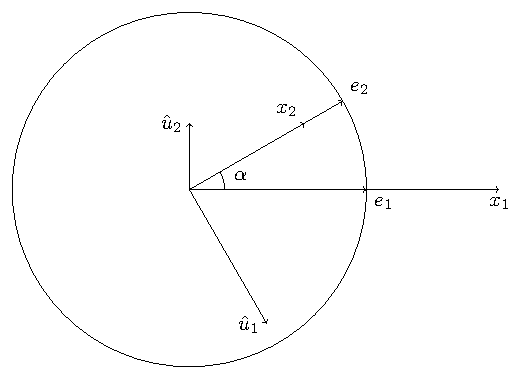
\includegraphics[width=0.3\linewidth]{figures/02_duality_first_residuals_translated.pdf}
\label{fig:duality_fst_residuals_translated}}
\subfigure[]{
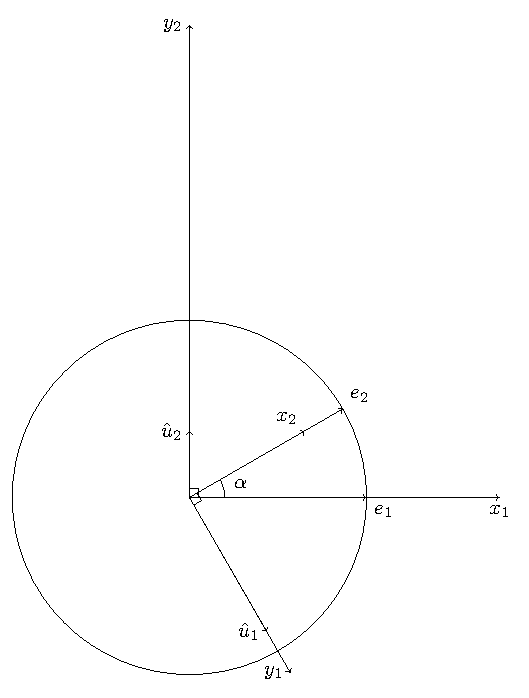
\includegraphics[width=0.3\linewidth]{figures/02_duality_new_regressors.pdf}
\label{fig:duality_new_regreesors}}
\subfigure[]{
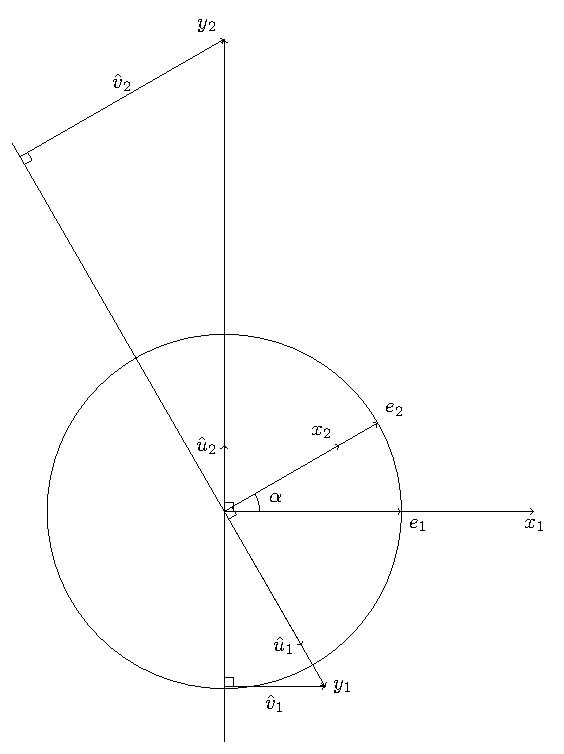
\includegraphics[width=0.3\linewidth]{figures/02_duality_new_residuals.pdf}
\label{fig:duality_new_residuals}}
\caption{\subref{fig:duality_fst_residuals_translated}: Residuals translated to the orgin of the unit circle;
\subref{fig:duality_new_regreesors}: Regressors $v_1$, $v_2$ obtained from inversion of the residuals $\hat{u}_1$, $\hat{u}_2$;
\subref{fig:duality_new_residuals}: Regressions of $v_1$ onto $v_2$ and of $v_2$ onto $v_1$.}
\end{center}
\end{figure*}

There two things to notice about the new residuals $\hat{v}_1$, $\hat{v}_2$.
First, $\hat{v}_1$ is perpendicular to the line spanned by $\tilde{e}_2$.
Similarly, $\hat{v}_2$ is perpendicular to the line spanned by $\tilde{e}_1$.
This means, that they are parallel to $e_1$, $e_2$ correspondingly
and once translated, they can be expressed as a multiple of $x_1$, $x_2$.

Second, we can find the lengths of these new residuals from the~right
triangles depicted in Figure~\ref{fig:duality_new_residuals}:
\begin{align*}
& \lVert \hat{v}_1 \rVert = \sin \alpha \cdot \lVert y_2 \rVert = \sin \alpha \cdot \left\lVert \frac{1}{\sin \alpha \cdot \lambda_1} \tilde{e}_1 \right\rVert = \frac{1}{\lambda_1} \\
& \lVert \hat{v}_2 \rVert = \sin \alpha \cdot \lVert y_1 \rVert = \sin \alpha \cdot \left\lVert \frac{1}{\sin \alpha \cdot \lambda_2} \tilde{e}_2 \right\rVert = \frac{1}{\lambda_2}
\end{align*}
Thus, when translated to the origin, the new resiuduals can be rewritten as
\begin{align*}
& \hat{v}_1 = \frac{1}{\lambda_1} e_1 \\
& \hat{v}_2 = \frac{1}{\lambda_2} e_2
\end{align*}

\begin{marginfigure}
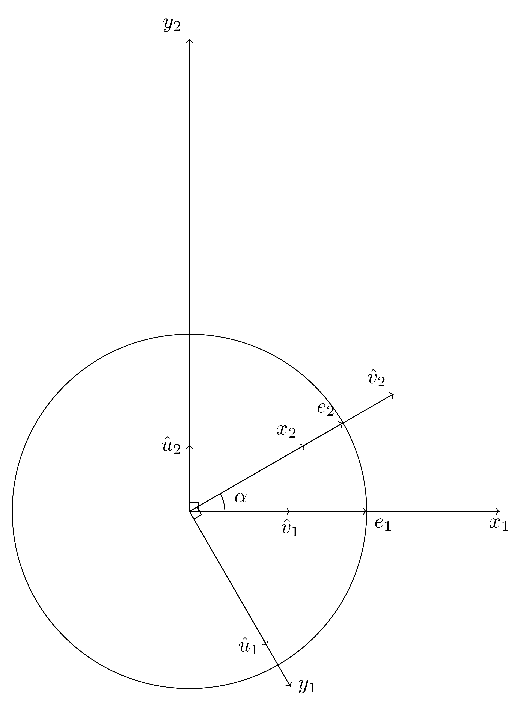
\includegraphics[scale=0.65]{figures/02_duality_final.pdf}
\label{fig:duality_final}
\caption{New residuals translated to the origin of the unit circle.}
\end{marginfigure}

The last step is to invert $\hat{v}_1$, $\hat{v}_2$.
Following the same procedure as described above, we finally get the desired result:
\begin{align*}
& \hat{v}_1 = \frac{1}{\lambda_1} e_1 \to \lambda_1 e_1 = x_1 \\
& \hat{v}_2 = \frac{1}{\lambda_2} e_2 \to \lambda_2 e_2 = x_2
\end{align*}
\end{proof}

\subsection{Gauss-Markov theorem}

% Hansen
\marginnote{
Consider an estimator $\beta$ which is a linear function of $Y$:
\[
\beta = A^T Y
\]
where $A$ is an $n \times k$ function of $X$ such that $A^T X = I_k$.
From
\begin{align*}
\Var(\hat\beta_{OLS}) &= (X^T X)^{-1} \sigma^2 \\
\Var(A^T Y) &= A^T A \sigma^2
\end{align*}
it follows that it is sufficient to prove that $A^T A - (X^T X)^{-1}$
is positive semi-definite. Set $C = A - X(X^T X)^{-1}$ and note that $X^T C = 0$, then
\begin{multline*}
A^T A - (X^T X)^{-1} \\
= (C + X(X^T X)^{-1})^T (C + X(X^T X)^{-1}) - (X^T X)^{-1} \\
= C^T C + C^T X(X^T X)^{-1} + (X^T X)^{-1} X^T C + \\
(X^T X)^{-1} X^T X(X^T X)^{-1} - (X^T X)^{-1} \\
= C^T C
\end{multline*}
Matrix $C^T C$ is positive semi-definite since
\[
\forall a \not= 0 \qquad a^T C^T C a = \lVert C a \rVert^2 \geq 0
\]
}

\begin{theorem}
In the homoskedastic linear regression model the best (minimum-variance) linear
unbiased estimator is given by the ordinary least squares.
\end{theorem}

\begin{proof}
Consider an OLS estimator and an alternative one:
\begin{align*}
\hat{\beta}_{OLS} &= (X^T X)^{-1} X^T y = A^T y \\
\hat{\beta}_{alt} &= A^T_{alt} y
\end{align*}
Note that $A^T X = I_{k}$, then the following holds for all $\beta$:
\begin{align*}
A^T X \beta &= \beta \\
A^T_{alt} X \beta &= \beta
\end{align*}
Taking the differnce of these equations, we obtain:
\[
(A^T_{alt} - A^T) X \beta = 0 \Rightarrow (A^T_{alt} - A^T) \perp X
\]
If we treat the coefficients separately and consider, for instance, $\beta^{(2)}$,
we get the following result
\[
({a^{(2)}}^T_{alt} - {a^{(2)}}^T) \perp X
\]
where $a^{(2)}_{alt}$ and $a^{(2)}$ are the second columns of matrices
$A_{alt}$ and $A$ correspondingly.
Since $a^{(2)} \in Lin(col X)$, it follows that $a^{(2)}_{alt} \not \in Lin(col X)$.

\begin{marginfigure}[3\baselineskip]
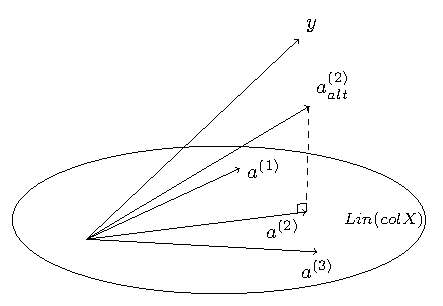
\includegraphics[scale=0.7]{figures/02_gmt.pdf}
\label{fig:gmt}
\caption{Gauss-Markov theorem for the case of three regressors.}
\end{marginfigure}

Now we can expxress the variances of both estimators in terms of $a^{(2)}_{alt}$ and $a^{(2)}$:
\begin{align*}
\Var\left(\hat{\beta}^{(2)}_{OLS}\right) &= \Var\left({a^{(2)}}^T y\right) = {a^{(2)}}^T \sigma^2 I_{k} a^{(2)} = \lVert a^{(2)} \rVert^2 \\
\Var\left(\hat{\beta}^{(2)}_{alt}\right) &= \Var\left({a^{(2)}}^T_{alt} y\right) =  {a^{(2)}}^T_{alt} \sigma^2 I_{k} a^{(2)}_{alt} = \lVert a_{alt}^{(2)} \rVert^2
\end{align*}
Since vectors $a^{(2)}$, $a^{(2)}_{alt}$ and $a^{(2)} - a^{(2)}_{alt}$
form a right triangle and $a^{(2)}_{alt} \not \in Lin(col X)$,
the vector $\lVert a_{alt}^{(2)} \rVert^2$ must be longer than $a^{(2)}$,
and the corresponding estimator must have higher variance.

\end{proof}
